%label:"art:IntroductionToLefschetz"
%type:"article"
%name:"introduction to Lefschetz fibrations in symplectic geometry"
%caption:""
%parent:""


We now explore Lagrangians $K\subset X$, where we have a projection $:X\to \CC$. 

%label:"def:symplecticLefschetzFibration"
%author:JeffHicks
%name:"symplectic lefschetz fibration"
%type:"definition"
%parent:"art_Lefschetz"
%source:"seidel2008fukaya"

\begin{definition}
    Let $(X, \omega , J)$ be a symplectic manifold equipped with compatible almost complex structure.
    A \emph{symplectic Lefschetz fibration} is map $\pi: X\to \CC$ satisfying the following properties:
    \begin{itemize}
        \item $\pi$ is $J$-holomorphic, in the sense that $J\pi_*=\pi_*\jmath$, where $\jmath$ is the standard complex structure on $\CC$;
        \item The map $\pi$ has finitely many critical points;
        \item The set of critical values $\{\pi(x)\;|\;z\in \Crit(\pi)\}$ are disjoint and;
        \item In a neighborhood of each critical point, there exists holomorphic coordinates $(z_1, \ldots, z_n)$ for $X$ so that $\pi=\sum_{i=1}^n z_i^2$. 
    \end{itemize}
    If the map $\pi$ is not proper (i.e. the fibers are allowed to be non-compact,) then we impose the additional requirement:
    \begin{itemize}
        \item There exists a compact set $X_0\subset X$ so that $\pi:X_0\to \CC$ is a proper fibration and;
        \item The fibration $\pi:X\setminus X_0\to \CC$ is a trivial symplectic fibration, with split complex and symplectic structure. 
    \end{itemize}
\end{definition}

Note that $\pi: X\times \CC\to \CC$, the setting considered for \snip{Lagrangian cobordisms}{def_lagrangianCobordism}, trivially satisfies these criterion. 
A symplectic Lefschetz fibration is the symplectic geometry equivalent to a manifold equipped with a Morse function.
The basic model that we consider is a function which models the neighborhood of a critical point.

%label:"exm:LocalModelOfASingularity"
%type:"example"
%name:"local model of a singularity"
%caption:""
%parent:"art_lefschetzExpanded"


    The symplectic fibration which we will use as a running example through this section is 
    \begin{align*}
        \pi:\CC^2\to& \CC\\
        (z_1, z_2)\mapsto& z_1z_2.
    \end{align*}
    This has one critical value at $z_1z_2=0$.
    The generic fiber $\pi^{-1}(z)$ is symplectomorphic to $(\CC^*)^2$.
    At the origin, this degenerates to the union of two complex lines, $\CC_{z_1=0}\cup \CC_{z_2=0}$.
    \cref{fig:ModelLefschetzSingularity} is a drawing of this Lefschetz fibration.


%label:"fig:ModelLefschetzSingularity"
%type:"figure"
%name:"model lefschetz singularity"
%caption:"The model Lefschetz singularity"
%parent:"art_lefschetzExpanded"


    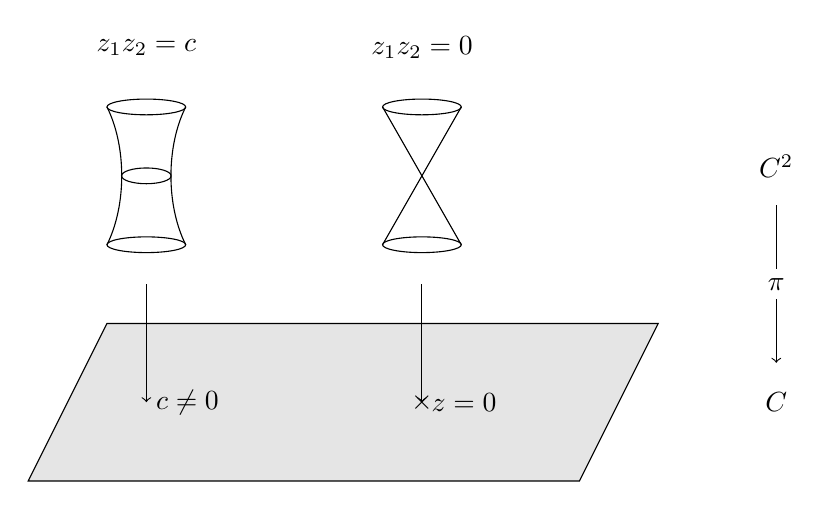
\begin{tikzpicture}
\draw[fill=gray!20] (-2.5,2.5) -- (-3.5,0.5) -- (3.5,0.5) -- (4.5,2.5) -- cycle;
\begin{scope}[scale=0.5, shift={(7,3.5)}]
\draw  (-4,7) ellipse (1 and 0.2);
\draw  (-4,3.5) ellipse (1 and 0.2);
\draw (-5,7) -- (-3,3.5) (-5,3.5) -- (-3,7);
\end{scope}
\begin{scope}[scale=0.5,shift={(0,3.5)}]
\draw  (-4,7) ellipse (1 and 0.2);
\draw  (-4,3.5) ellipse (1 and 0.2);

\draw (-5,7) .. controls (-4.5,6) and (-4.5,4.5) .. (-5,3.5);
\draw (-3,7) .. controls (-3.5,6) and (-3.5,4.5) .. (-3,3.5);
\draw  (-4,5.25) ellipse (0.63 and 0.2);
\end{scope}

\draw[->] (-2,3) -- (-2,1.5);
\draw[->](1.5,3) -- (1.5,1.5);
\node at (1.5,1.5) {$\times$};
\node[right] at (1.5,1.5) {$z=0$};
\node[right] at (-2,1.5) {$c\neq 0$};
\node at (6,1.5) {$\mathbb C$};
\node at (6,4.5) {$\mathbb C^2$};
\draw[->] (6,4) -- (6,2);
\node[fill=white] at (6,3) {$\pi$};
\node at (1.5,6) {$z_1z_2=0$};
\node at (-2,6) {$z_1z_2=c$};
    \label{fig:modelsingularity}

\end{tikzpicture}
%label:"exm:CotangentBundleOfASphere"
%type:"example"
%name:"cotangent bundle of a sphere"
%caption:""
%parent:"art_lefschetzExpanded"


    Another interesting piece of geometry comes from the cotangent bundle of the 2-sphere, which is a subvariety of $\CC^{3}$,
    \[T^*S^2=\{(z_0, z_1, z_2)\;|\; z_0^2+z_1^2+z_2^2=1\}\]
    We check that this has the topology of the tangent bundle.
    Let $S^2=\{(x_0, x_1, x_2)\;|\; x_0^2+x_1^2+x_2^2=1\}\subset \RR^3$. 
    The tangent bundle is then described by the pairs 
    \[T^*S^2:=\{(x_0, x_1, x_2, y_0, y_1, y_2)\;|\;x_0^2+x_1^2+x_2^2=1, \sum_{i=0}^2 x_iy_i=0 \}.\]
    These two constraints can be rephrased in terms of the real and imaginary components of $z_0^2+z_1^2+z_2^2=1$. 
    The complex structure on this cotangent bundle interchanges the $x_i$ base directions with the $y_i$ tangent bundle directions.
    The symplectic Lefschetz fibration that we consider for the cotangent bundle of the sphere sends 
    \begin{align*}
        \pi: T^*S^2\to \CC\\
        (z_0, z_1, z_2)\mapsto z_2
    \end{align*}
    The fibers of this function are the conics 
    \[\pi^{-1}(z)=\{(z_0, z_1, z_2)\;|\; z_2=z, z_0^1+z_1^2=1-z_2^2\}\]
    which are regular, provided that $z_2\neq \pm 1$. 
%label:"fig:LefschetzFibrationForCotangentBundleOfASphere"
%type:"figure"
%name:" Lefschetz fibration for cotangent bundle of a sphere"
%caption:"Lefschetz fibration for the cotangent bundle of the sphere"
%parent:""

        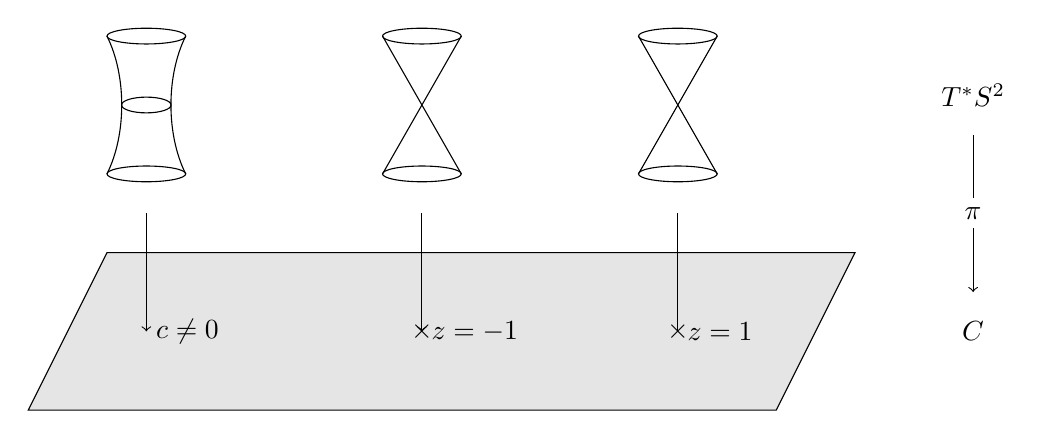
\begin{tikzpicture}

\draw[fill=gray!20] (-2.5,2.5) -- (-3.5,0.5) -- (6,0.5) -- (7,2.5) -- cycle;
\begin{scope}[scale=0.5, shift={(7,3.5)}]
\draw  (-4,7) ellipse (1 and 0.2);
\draw  (-4,3.5) ellipse (1 and 0.2);
\draw (-5,7) -- (-3,3.5) (-5,3.5) -- (-3,7);
\end{scope}
\begin{scope}[scale=0.5, shift={(13.5,3.5)}]
\draw  (-4,7) ellipse (1 and 0.2);
\draw  (-4,3.5) ellipse (1 and 0.2);
\draw (-5,7) -- (-3,3.5) (-5,3.5) -- (-3,7);
\end{scope}
\begin{scope}[scale=0.5,shift={(0,3.5)}]
\draw  (-4,7) ellipse (1 and 0.2);
\draw  (-4,3.5) ellipse (1 and 0.2);

\draw (-5,7) .. controls (-4.5,6) and (-4.5,4.5) .. (-5,3.5);
\draw (-3,7) .. controls (-3.5,6) and (-3.5,4.5) .. (-3,3.5);
\draw  (-4,5.25) ellipse (0.63 and 0.2);
\end{scope}

\draw[->] (-2,3) -- (-2,1.5);
\draw[->](1.5,3) -- (1.5,1.5);
\node at (1.5,1.5) {$\times$};
\node[right] at (1.5,1.5) {$z=-1$};
\node at (4.75,1.5) {$\times$};
\node[right] at (4.75,1.5) {$z=1$};
\node[right] at (-2,1.5) {$c\neq 0$};
\node at (8.5,1.5) {$\mathbb C$};
\node at (8.5,4.5) {$T^*S^2$};
\draw[->] (8.5,4) -- (8.5,2);
\node[fill=white] at (8.5,3) {$\pi$};


\draw (4.75,3) -- (4.75,1.5);
\end{tikzpicture}



\begin{remark}
    One slightly confusing piece of notation in symplectic geometry is that the tangent bundle of $\CP^1$ is usually equipped with a different symplectic form that the cotangent bundle $T^*S^2$.
    This is because $T\CP^1$ is usually considered with the symplectic form which makes $\CP^1$ a symplectic, rather than Lagrangian submanifold.
    This can also be constructed as the symplectic blowup of $\CC^2$ at the origin.
    This also comes with a projection to $\CC$, by first considering the blowdown map $T\CP^1\to \CC^2$, and then composing with the fibration considered in \cref{exm:LocalModelOfASingularity}.
    This is not a Lefschetz fibration, as the critical fiber above zero contains 2 critical points.
\end{remark}
The existence of a \emph{symplectic parallel transport map} across the fibers of a Lefschetz fibration allows us to carry over many of the constructions which we considered for Lagrangian cobordisms to Lefschetz fibrations.
%label:"prp:SymplecticParallelTransport"
%type:"proposition"
%name:"symplectic parallel transport"
%caption:""
%parent:"art_lefschetzExpanded"


    The regular fibers $X_z:=\pi^{-1}(z)$ of $\pi$ are symplectic submanifolds, and there exists a connection on $TX$ whose parallel transport is a symplectomorphism of the fibers. 


%label:"prf:SymplecticParallelTransport"
%type:"proof"
%name:"symplectic parallel transport"
%caption:""
%parent:""


    We first show that $\ker(\pi_*)$ is a symplectic subspace. 
    Let $0\neq v\in \ker(\pi_*)$ be any tangent vector.
    Since $\pi_*$ is $J$-holomorphic, $Jv\in \ker(\pi_*)$. 
    We conclude that $\omega(v, Jv)=g(v, v)\neq 0$, and so $\omega$ is non-degenerate on the subspace $\ker(\pi_*)=T_zX$. 
    It remains to show that the form is closed. 
    Let $i:X_z\into X$ be and inclusion of a fiber of the Lefschetz fibration.
    Then $di^*\omega= i^*d\omega =0$, so the $\omega|_{X_z}$ is a symplectic form on the fiber. 

    We can construct a connection by picking a horizontal complement to the kernel of the projection. 
    As $\ker(\pi_*)$ is a symplectic subspace, $(\ker(\pi_*))^{\omega\bot}$, its symplectic complement, is a complementary subspace in the sense that $\ker(\pi_*)\oplus (\ker(\pi_*))^{\omega\bot}=TX$. 
    This is a choice of horizontal complement, defining a connection on this fiber bundle. 
    In fact, the splitting of the tangent bundle locally splits the symplectic form. 
%label:"prp:LocalSymplecticFormInLefschetzFibration"
%type:"proposition"
%name:"local symplectic form in Lefschetz fibration"
%caption:""
%parent:"prf_SymplecticParallelTransport"


    In the local splitting $T_xX=\ker(\pi_*)\oplus(\ker(\pi_*))^{\omega^\bot}$, the symplectic form $\omega_X$ can be written as  
    \[\omega_X=\omega|_{X_z}\oplus f\omega_\CC.\]
    for some smooth function $f:X\to \RR$.



%label:"prf:LocalSymplecticFormInLefschetzFibration"
%type:"proof"
%name:"local symplectic form in Lefschetz fibration"
%caption:""
%parent:""


    Pick $p\in X$ a point, and tangent vectors  $(v_1, w_1), (v_2, w_2)\in T_pX=\ker(\pi_*)\oplus(\ker(\pi_*))^{\omega^\bot}.$ 
    Because this these two spaces are symplectic orthogonal, $\omega_X(v_1, w_2)=0$ and $\omega_X(v_2, w_1)=0$. 
    Since $v_1, v_2$ are tangent vectors to $X_p$, and symplectic forms on $\CC$ are all scalar multiples, there exists a function $f: X\to \RR$ yielding the decomposition
    \begin{align*} 
    \omega_X((v_1, w_1), (v_2, w_2))=&\omega_X((v_1, 0), (v_2, 0))+ \omega_X((0, w_1), (0, w_2)).
    =&\omega_{X_p}(v_1, v_2)+f(p) \pi^*\omega_\CC(w_1, w_2)
    \end{align*}






    We now show that parallel transport is a symplectomorphism of the fibers.
    This is done by computing the vertical component of the Lie derivative of $\omega$. 
    Let $v\in \ker(\pi_*)^{\omega \bot}$ be a horizontal vector. 
    Then 
    \[\mathcal L_{v \omega}=d\iota_v \omega\]
    We note that $\iota_v\omega$ vanishes on vertical vectors.
    Therefore, $d\iota_v\omega$ vanishes on pairs of vertical vectors, and so the vertical component of the Lie derivative of $\omega$ is zero. 
    This allows us to make the following definition.
%label:"def:SymplecticParallelTransportMap"
%type:"definition"
%name:"symplectic parallel transport map"
%caption:""
%parent:"art_lefschetzExpanded"


        Let $\gamma:[0,1]_t\to X\setminus \Crit(\pi)$.
        Define the symplectomorphism $\phi_\gamma^t: X_{\gamma(0)}\to X_{\gamma(t)}$ to be the symplectic parallel transport along the path $\gamma$. 
        Define the symplectic inclusion $i_\gamma^t: X_{\gamma(0)}\to X$ to be the symplectic parallel transport map composed with the inclusion of the fiber into the total space $X$.


    Finally, we prove that the autosymplectomorphism of the fiber taken by small loops are Hamiltonian isotopies. .
    Suppose that we have a family of loops $\gamma_s:[0,1]_s\times [0,1]_t\to \CC$ with $\gamma_s(0)=\gamma_s(1)=\gamma_1(t)=z$.
    This gives us a family of maps $i_\gamma^t: X_z\into X$  and a symplectomorphisms $\phi_{s, 1}: X_z\to X_z$. 
    Let $c:S^1\to X_{z}$ represent a class in $H_1(X_z)$, and consider the flux $\int_{\phi_{s, 1}\circ c}\omega|_{X_z}$. 
    We can write this chain as the boundary of a 3 chain, 
    \[c\times [0, 1]_s\times\{t=1\}\cup c\times [0, 1]_s\times \{t=0\}\cup c\times \{0\}_s \times [0, 1]_t\cup c\times \{1\}_s\times [0, 1]_t=\partial (c\times [0, 1_s]\times [0, 1]_t)\]
    This allows us to replace the flux integral with 
    \begin{align*}
        0=&\int_{i_\gamma^t\circ c} d\omega = \int_{\partial(i_\gamma^t\circ c)}\omega\\
        =& \int_{i{s, 1}\circ c}\omega-\int_{i{s, 0}\circ c}\omega+\int_{i{1, t}\circ c}\omega-\int_{i_{0, t}\circ c}\omega
        \intertext{The first term is an integral restricted to the fiber $X_z$, so we may replace $\omega$ with $\omega|_{X_z}$. The second term and fourth term are  zero as the map is constant. }
        =& \int_{i{s, 1}\circ c}\omega|_{X_z}+\int_{i{1, t}\circ c}\omega\\
        \intertext{In the last term $\frac{d}{dt}i_{1, t}\circ c$ lies in the horizontal tangent space, and $\frac{d}{d\theta} i_{1,t}\circ c$ lies in the vertical tangent space. Therefore $\omega$ vanishes on $T(i_{1, t}\circ c)$ }
        =&\int_{i{s, 1}\circ c}\omega|_{X_z}= \Flux_{i_{s, 1}}(c).
    \end{align*}
\end{proof}
%label:"prp:ParallelTransportOfLagrangianSubmanifold"
%type:"proposition"
%name:"parallel transport of Lagrangian submanifold"
%caption:""
%parent:"art_lefschetzExpanded"


    Consider a symplectic Lefschetz fibration $\pi: X\to \CC$. 
    Let $\gamma:\RR\to \CC$ be a path avoiding the critical values of a symplectic Lefschetz fibration. 
    Additionally, pick a Lagrangian submanifold  of a fiber $L\subset X_{\gamma(0)}$, parameterized by $\li: L\to X$.  
    Consider the submanifold $K$ parameterized by 
    \begin{align*}\li_t: L\times \RR\to& X\\
        (x, t) \mapsto&  (i\gamma^t\circ \li(x))
    \end{align*} 
    where $i_\gamma^t: X_{\gamma_0}\to X$ is given by parallel transport along $\gamma$. 
    $K$ is a Lagrangian submanifold of $X$. 


%label:"prf:ParallelTransportOfLagrangianSubmanifold"
%type:"proof"
%name:"parallel transport of Lagrangian submanifold"
%caption:""
%parent:""


    Let $\li_t:L\times \RR\to X$ be a parameterization of the submanifold $K$.
    By reparameterization, it suffices to check that this is a Lagrangian submanifold at points $(p, 0)$. 
    The tangent space $T_{(p, 0)}(L\times \RR)$ is spanned by vectors $\{\partial_{x_1}, \ldots, \partial_{x_{n-1}}, \partial_t\}$. 
    Because $L$ is a Lagrangian of the fiber, and the fiber is a symplectic submanifold,
    \[\li_t^*\omega(\partial_{x_i}, \partial_{x_j})=0.\]
    Since $K$ was constructed via parallel transport, $(\li_t)_*\partial_t\in (\ker(\pi_*))^{\omega\bot}$. Since $L$ is a Lagrangian of the fiber, $(\li_t)_*\partial_{x_i}\in \ker(\pi_*)$.
    Therefore, 
    \begin{align*}\li_t^*\omega(\partial_{x_i}, \partial_{t})=0
    \end{align*}


%label:"fig:ProductTorus"
%type:"figure"
%name:"product torus"
%caption:"Product Torus constructed via Lefschetz fibration"
%parent:"art_lefschetzExpanded"


        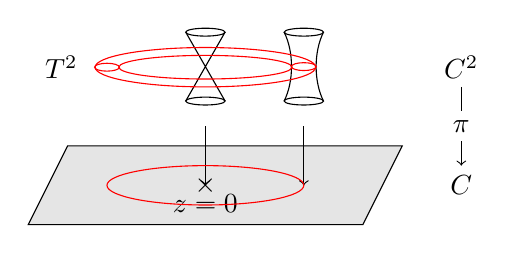
\begin{tikzpicture}[scale=.5]

\draw[fill=gray!20] (-2.5,2.5) -- (-3.5,0.5) -- (5,0.5) -- (6,2.5) -- cycle;
\begin{scope}[scale=0.5, shift={(6,3.78)}]
\draw  (-4,7) ellipse (1 and 0.2);
\draw  (-4,3.5) ellipse (1 and 0.2);
\draw (-5,7) -- (-3,3.5) (-5,3.5) -- (-3,7);
\end{scope}

\begin{scope}[scale=0.5,shift={(11,3.78)}]
\draw  (-4,7) ellipse (1 and 0.2);
\draw  (-4,3.5) ellipse (1 and 0.2);

\draw (-5,7) .. controls (-4.5,6) and (-4.5,4.5) .. (-5,3.5);
\draw (-3,7) .. controls (-3.5,6) and (-3.5,4.5) .. (-3,3.5);
\draw[red]  (-4,5.25) ellipse (0.63 and 0.2);
\end{scope}

\draw[->] (3.5,3) -- (3.5,1.5);
\draw[->](1,3) -- (1,1.5);
\node at (1,1.5) {$\times$};
\node[below] at (1,1.5) {$z=0$};


\node at (7.5,1.5) {$\mathbb C$};
\node at (7.5,4.5) {$\mathbb C^2$};
\draw[->] (7.5,4) -- (7.5,2);
\node[fill=white] at (7.5,3) {$\pi$};





\node[left] at (-2,4.5) {$T^2$};

\draw[red, scale=.5]  (-3,9) ellipse (0.63 and 0.2);

\draw[red]  (1,4.5) ellipse (2.8 and 0.5);
\draw[red]  (1,4.5) ellipse (2.2 and 0.3);
\draw[red]  (1,1.5) ellipse (2.5 and 0.5);

\end{tikzpicture}

%label:"fig:ChekanovTorus"
%type:"figure"
%name:" Chekanov torus"
%caption:"Chekanov Torus constructed via Lefschetz fibration"
%parent:"art_lefschetzExpanded"


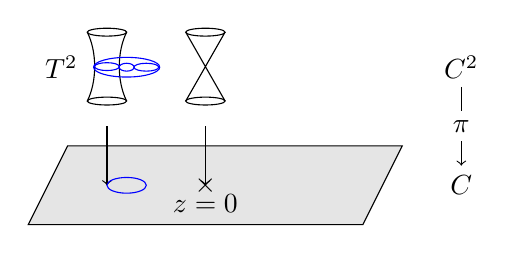
\begin{tikzpicture}[scale=.5]

\draw[fill=gray!20] (-2.5,2.5) -- (-3.5,0.5) -- (5,0.5) -- (6,2.5) -- cycle;
\begin{scope}[scale=0.5, shift={(6,3.78)}]
\draw  (-4,7) ellipse (1 and 0.2);
\draw  (-4,3.5) ellipse (1 and 0.2);
\draw (-5,7) -- (-3,3.5) (-5,3.5) -- (-3,7);
\end{scope}

\begin{scope}[scale=0.5,shift={(1,3.78)}]
\draw  (-4,7) ellipse (1 and 0.2);
\draw  (-4,3.5) ellipse (1 and 0.2);

\draw (-5,7) .. controls (-4.5,6) and (-4.5,4.5) .. (-5,3.5);
\draw (-3,7) .. controls (-3.5,6) and (-3.5,4.5) .. (-3,3.5);
\draw[blue]  (-4,5.25) ellipse (0.63 and 0.2);
\end{scope}

\draw[->] (-1.5,3) -- (-1.5,1.5);
\draw[->](1,3) -- (1,1.5);
\node at (1,1.5) {$\times$};
\node[below] at (1,1.5) {$z=0$};


\node at (7.5,1.5) {$\mathbb C$};
\node at (7.5,4.5) {$\mathbb C^2$};
\draw[->] (7.5,4) -- (7.5,2);
\node[fill=white] at (7.5,3) {$\pi$};





\node[left] at (-2,4.5) {$T^2$};

\draw[blue]  (-1,4.5) ellipse (0.19 and 0.1);
\draw[blue, scale=.5]  (-1,9) ellipse (0.63 and 0.2);
\draw[blue]  (-1,4.5) ellipse (.84 and 0.25);
\draw[blue]  (-1,1.5) ellipse (0.5 and 0.2);

\end{tikzpicture}
When we have a curve $\gamma: \RR\to \CC$ which avoids the critical values, and a Lagrangian submanifold $L\subset X_{\gamma(0)}$, we will abuse notation and denote the parallel transport of $L$ along $\gamma$ by $L\times \gamma$. 
%label:"exm:LagrangiansGivenBySymplecticParallelTransport"
%type:"example"
%name:"Lagrangians given by symplectic parallel transport"
%caption:""
%parent:"art_lefschetzExpanded"


    Recall our running example $\pi:\CC^2\to \CC$ from \cref{exm:LocalModelOfASingularity}. 
    We will prove that the symplectic parallel transport map preserves a class of Lagrangian submanifolds of the fiber.
    Consider the function $H(z_1, z_2)= \frac{1}{2}\left(|z_1|^2-|z_2|^2\right)=\frac{1}{2}\left( x_1^2+y_1^2-x_2^2-y_2^2\right)$. 
    The exterior derivative of this function, in local coordinates, is given by 
    \[dH= x_1dx_1 +y_1dy_1 -x_2dx_2- y_2dy_2.\]
    We prove that $H$ is invariant under the action of symplectic parallel transport along the fibration $\pi:\CC^2\to \CC$. 
    In this example, we can explicitly compute that $H$ is invariant under vectors contained in $\ker(d\pi)^{\omega_\bot}$. 
    
    The kernel of $d\pi=z_2dz_1+z_1dz_2$ at a point $(z_1, z_2)$ is the complex subspace generated by the vector \begin{align*}
        \ker_{(z_1, z_2)}(d\pi)=&\Span_\CC(\langle z_1, -z_2\rangle)\\
        =&\Span_\RR(\langle x_1, y_1, -x_2, -y_2\rangle, \langle -y_1, x_1, y_2, -x_2\rangle ).
    \end{align*}
    In this setting, the symplectic complement is described by the orthogonal complement, and so 
    \begin{align*}
        (\ker_{(z_1, z_2)}(d\pi))^{\omega\bot}=&\Span_\CC(\langle \bar z_2, \bar z_1\rangle)\\
        =&\Span_\RR(\langle x_2, -y_2, x_1, -y_1\rangle, \langle y_2, x_2, y_1, x_1\rangle ).
    \end{align*}
    One then checks that $dH$ vanishes on this by computing $dH(v)=0$ for $v\in (\ker_{(z_1, z_2)}(d\pi))^{\omega\bot}$
    \begin{align*}
        \langle x_1, y_1, -x_2,- y_2\rangle\cdot \langle x_2, -y_2, x_1, -y_1\rangle=&0\\
        \langle x_1, y_1, -x_2,-y_2\rangle\cdot \langle y_2, x_2, y_1, x_1 \rangle=&0
    \end{align*}

    This means that the level sets of $H$ are preserved under parallel transport.
    We use to this to describe some Lagrangian submanifolds of $\CC^2$. 

    If we take a level set of $H$ and restrict to a fiber above the point $re^{\jmath c}$, the level set $H^{-1}(\lambda)\cap \pi^{-1}(re^{\jmath c})$ can be explicitly parameterized by $S^1:=\theta\mapsto re^{\jmath c}\cdot(s e^{\jmath\theta}, s^{-1} e^{-\jmath\theta})$, where $s$ is determined by $r^2(s^2-s^{-2})=\lambda$. 
    Simply because every curve is a Lagrangian submanifold of a $\CC^*$, the level set of $H$ restricted to a fiber of $\pi$ is a Lagrangian submanifold.
    
    We can now apply \cref{prp:ParallelTransportOfLagrangianSubmanifold} to obtain some new Lagrangian submanifolds of $\CC^2$ from parallel transport of these level sets. 
    Let $\gamma:[0, 1]\to \CC\setminus 0$ be a closed curve, and $\lambda\in \RR$ some value. 
    Define the Lagrangian $L_{\gamma, \lambda}$ to be the parallel transport of the $\lambda$-level set along the curve $\gamma$. 
    This already gives several interesting examples of Lagrangian submanifolds inside of $\CC^2$. 
    These Lagrangian submanifolds can also be characterized in the following way:
    \[L_{\gamma, \lambda}:=\{(z_1, z_2)\;|\; H(z_1, z_2)=\lambda, \pi(z_1, z_2)\in \Im(\gamma)\}.\]

    A good example of one of these Lagrangians is the \emph{product torus}. Let $\gamma_r=re^{\jmath\theta}$.
    Let $s$ be the real value so that $r^2(s^2-s^{-2})=\lambda$.  Then the Lagrangian $L_{\gamma_r, \lambda}$ is explicitly parameterized by:
    \[L_{\gamma_r, \lambda}=\{r(se^{\jmath\theta_1}, se^{\jmath\theta_2})\}\]
    This agrees with the definition of the product torus from \cref{exm:productTorus}.


A Lefschetz fibration $\pi: X\to \CC$ equips $X$ with two Hamiltonian flows: the real and imaginary coordinates of the complex parameter. 

%label:"lem:GradientOfRealPartInLefschetzFibration"
%type:"lemma"
%name:"gradient of real part in Lefschetz fibration"
%caption:""
%parent:"art_lefschetzExpanded"


    Let $\pi: X\to \CC$ be a symplectic Lefschetz fibration. Let $g_X=\omega_X\circ (J_X\tensor \id)$ be the compatible metric on $X$.
    Then we have the following relations between gradient and Hamiltonian flows. 
    \begin{itemize}
        \item The gradient flow of $\pi_\RR$ is the Hamiltonian flow of $\pi_{i\RR}$. 
        \item The gradient flow of $\pi_{i\RR}$ is the Hamiltonian flow of $-\pi_\RR$. 
	\end{itemize}


%label:"prf:GradientOfRealPartInLefschetzFibration"
%type:"proof"
%name:"gradient of real part in Lefschetz fibration"
%caption:""
%parent:""


    This follows from \cref{lem:gradients}.


%label:"prp:LocelModelOfThimble"
%type:"proposition"
%name:"locel model of thimble"
%caption:""
%parent:"art_lefschetzExpanded"


    Let $p\in \Crit(\pi)$ be a critical point of a symplectic Lefschetz fibration. 
    Consider the function $\Re(\pi):X\to \RR$. 
    The point $p$ is also critical point of $\Re(\pi)$ and 
     $W^-_p$, the downward flow space of $p$, is a Lagrangian submanifold.  


%label:"prf:LocelModelOfThimble"
%type:"proof"
%name:"locel model of thimble"
%caption:""
%parent:""


    In the local model at a critical point of $\pi$, projection to the real coordinate can be written in local holomorphic coordinates as 
    \[\Re(\pi)=x_1^2+\ldots x_n^2-y_1^2-\ldots y_n^2.\]
    The downward flow space is parameterized by 
    \[W^-_p=\{x_1=y_1, \ldots, x_n=y_n\}\]
    which is a Lagrangian submanifold for the standard symplectic structure. 


%label:"exm:LagrangianThimble"
%type:"example"
%name:"lagrangian thimble"
%caption:""
%parent:"art_lefschetzExpanded"


    Once again we consider the Lefschetz fibration  $\pi: \CC^2\to \CC$ from \cref{exm:LocalModelOfASingularity}. 
    The only critical value of this function is $0$. 
    Given a path $\gamma:[0, 1]\to \CC$ with $\gamma(0)=0$, the thimble can be described by the construction of \cref{exm:LagrangiansGivenBySymplecticParallelTransport},
    \[D^n_\gamma=L_{\gamma, 0}.\]
    In particular case of $\gamma$ being the real positive $\RR_{\geq0}\subset \CC$,
    \begin{align*}
        L_{\gamma, 0}=&\{(z_1, z_2)\;|\;z_1z_2\in \RR_{\geq 0}, |z_1|^2-|z_2|^2=0\}\\
        =&\{(z, \bar z)\;|\; z\in \CC\}.
    \end{align*}


Note that $\pi(W^-_p)$ is a ray emerging from $\pi(p)$ and heading in the positive real direction. 
Let $z$ be in the interior of $\pi(W^-_p)$. 
Then $\pi^{-1}(z)\cap W^-_p$ is a Lagrangian sphere $S^{n-1}\subset \pi^{-1}(z)$. 
More generally, one can take any path $\gamma\subset \CC$ with left end on a critical endpoint to determine a Lagrangian sphere in the fiber. 
Note that the map  $(\phi_\gamma^{t_0})^{-1}: X_{\gamma(t_0)}\to X_{\gamma(0)}$ is still a well defined map. 
One can check that  $(\phi_{\gamma}^{t_0})^{-1}(z)\subset X_{\gamma(0)}$ is a Lagrangian sphere in the fiber. 
%label:"def:LagrangianThimble"
%type:"definition"
%name:"Lagrangian thimble"
%caption:""
%parent:"art_lefschetzExpanded"


    Let $\pi: X\to \CC$ be a symplectic fibration. 
    Let $\gamma:[0, 1]\to \CC$ be path with $\gamma(0)$ a critical value. Let $p$ be the critical point above this critical value. 
    Suppose $\gamma(t)$ avoids critical values for $t\neq 0$. 
    Let $W^{-1}(\gamma)$ be the collection of fibers above the path $\gamma$.
    Consider the map $(\phi_{\gamma}^{t})^{-1}:W^{-1}(\gamma)\mapsto X_{\gamma(0)}$ given by parallel transport.
    Then the \emph{thimble of $\gamma$ from $p$} is a Lagrangian disk $D^n_\gamma:= (\phi_{\gamma}^{t})^{-1}(z)\subset W^{-1}(\gamma)\subset X$.
    The \emph{vanishing cycle of $\gamma$} is a Lagrangian sphere $S^{n-1}_\gamma (\phi_{\gamma}^{1})^{-1}(z)\subset X_{\gamma(0)}$, which may also be identified with $ D^n_\gamma\cap  \pi^{-1}(\gamma(1))$. 


Sometimes, a sphere in the fiber is the vanishing cycle of more than one critical point.
If $\gamma_1, \gamma_2$ are two paths so that $S^{n-1}_{\gamma_1}=S^{n-1}_{\gamma_2}$, whose concatenation $\gamma=\gamma_1\cdot \gamma_2^{-1}$ is a smooth path, we call $\gamma$ a \emph{matching path} for the critical values $\gamma_1(0)$ and $\gamma_2(0)$. 
When we have a matching path, we can construct a Lagrangian sphere by gluing the corresponding thimbles together at their mutual vanishing cycle boundary.
%label:"exm:MatchingPathsInCotangentBundleOfTheSphere"
%type:"example"
%name:"matching paths in cotangent bundle of the sphere"
%caption:""
%parent:"art_lefschetzExpanded"


    We continue our discussion of the sphere from \cref{exm:CotangentBundleOfASphere}. 
    The Lefschetz fibration $\pi: T^*S^2\to S^2$ has two critical values, $\{-1, 1\}$, whose critical points corresponding to the north and south pole of the sphere. We now look at the thimbles drawn in \cref{fig:VanishingPathsForTheCotangentBundleOfTheSphere}.

    The first example we consider is the Lagrangian thimble constructed from $\gamma(t)=-1-t$, the real negative ray with endpoint on the critical value of the south pole.
    The symplectic parallel transport along $\gamma(t)$ is the negative gradient flow of the imaginary coordinate of $\pi(z_0, z_1, z_2)=z_2$ from the critical point $(0,0,1)$. 
    The gradient flow of the imaginary coordinate is 
    \begin{align*}
        \grad_{T^*S^2}(\Im(z_2))=&\text{proj}_{T(T^*S^2)}\grad_{\CC^3}(\Im(z_2))\\
        =&\langle 0, 0, 1 \rangle-  \cdot\frac{ \langle 0, 0, 1 \rangle\cdot \langle 2z_0, 2z_1, 2z_2 \rangle }{(2z_0)^2+(2z_1)^2+(2z_2)^2}\langle 2z_0, 2z_1, 2_2\rangle\\
        =&  h(z_0, z_1, z_2)\langle 0, 0, 1\rangle
    \end{align*}
    For some function $h(z_0, z_1, z_2)$. 
    The space $\{(ix_0, ix_1, 1+x_0^2+x_1^2)\}$ is a 2-dimensional Lagrangian subspace which contains $(0,0, 1)$ and is parallel to the $\grad_{T^*S^2}(\Im(z_2))$, and therefore the Lagrangian thimble over $\gamma(t)$. 
    This also corresponds to the cotangent fiber above the south pole, $T^*_{sp}S^2$.
    
    In this example, we can also consider the path $\gamma(t)=1-2t$, which starts at the critical value for the south pole and ends at the critical value of the north pole. 
    This is a matching path, and therefore there is a Lagrangian $S^2_{\gamma}\subset T^*S^2$ which lives above this path. 
    The zero section of the sphere, given by $\{(x_0, x_1, x_2)\;|\; x_0^2+x_1^2+x_2^2=1, x_i\in \RR\}$ is a 2 dimensional submanifold of $T^*S^2$ which lies parallel to $\grad_{T^*S^2}(\Im(z_2))$.
    The image of the zero section under $\pi$ is the curve $\gamma$, and the $S^2$ zero section clearly contains the north and south pole.
    Therefore, the Lagrangian sphere associated to the mapping path $\gamma$ is exactly the zero section. 


%label:"fig:VanishingPathsForTheCotangentBundleOfTheSphere"
%type:"figure"
%name:" vanishing paths for the cotangent bundle of the sphere"
%caption:"The matching math in the example of $\pi: T^*S^2\to \CC$ gives a Lagrangian sphere. The vanishing cycle above $0$ corresponds to the equator of the sphere."
%parent:"art_lefschetzExpanded"


    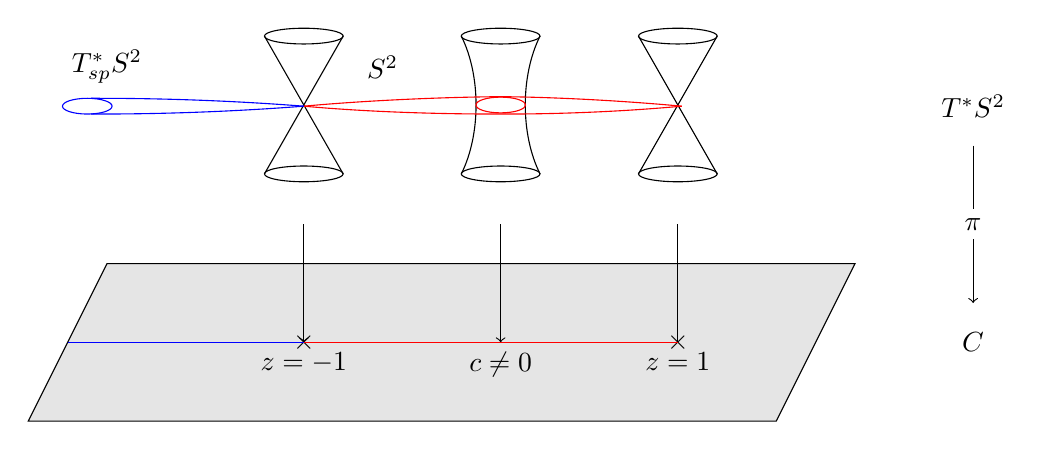
\begin{tikzpicture}

\draw[fill=gray!20] (-2.5,2.5) -- (-3.5,0.5) -- (6,0.5) -- (7,2.5) -- cycle;
\begin{scope}[scale=0.5, shift={(4,3.78)}]
\draw  (-4,7) ellipse (1 and 0.2);
\draw  (-4,3.5) ellipse (1 and 0.2);
\draw (-5,7) -- (-3,3.5) (-5,3.5) -- (-3,7);
\end{scope}
\begin{scope}[scale=0.5, shift={(13.5,3.78)}]
\draw  (-4,7) ellipse (1 and 0.2);
\draw  (-4,3.5) ellipse (1 and 0.2);
\draw (-5,7) -- (-3,3.5) (-5,3.5) -- (-3,7);
\end{scope}
\begin{scope}[scale=0.5,shift={(9,3.78)}]
\draw  (-4,7) ellipse (1 and 0.2);
\draw  (-4,3.5) ellipse (1 and 0.2);

\draw (-5,7) .. controls (-4.5,6) and (-4.5,4.5) .. (-5,3.5);
\draw (-3,7) .. controls (-3.5,6) and (-3.5,4.5) .. (-3,3.5);
\draw[red]  (-4,5.25) ellipse (0.63 and 0.2);
\end{scope}

\draw[->] (2.5,3) -- (2.5,1.5);
\draw[->](0,3) -- (0,1.5);
\node at (0,1.5) {$\times$};
\node[below] at (0,1.5) {$z=-1$};
\node at (4.75,1.5) {$\times$};
\node[below] at (4.75,1.5) {$z=1$};
\node[below] at (2.5,1.5) {$c\neq 0$};
\node at (8.5,1.5) {$\mathbb C$};
\node at (8.5,4.5) {$T^*S^2$};
\draw[->] (8.5,4) -- (8.5,2);
\node[fill=white] at (8.5,3) {$\pi$};


\draw (4.75,3) -- (4.75,1.5);
\draw[red] (0,4.5) .. controls (1.1,4.6) and (2.2,4.62) .. (2.5,4.62) .. controls (2.8,4.62) and (3.7,4.6) .. (4.8,4.5);

\draw[red,yscale=-1] (0,-4.5) .. controls (1.1,-4.4) and (2.2,-4.4) .. (2.5,-4.4) .. controls (2.8,-4.4) and (3.7,-4.4) .. (4.8,-4.5);
\draw[red] (0,1.5) -- (4.75,1.5);
\node at (1,5) {$S^2$};
\draw[blue] (0,1.5) -- (-3,1.5);

\draw[blue, scale=.5]  (-5.5,9) ellipse (0.63 and 0.2);

\draw[blue] (0,4.5) .. controls (-1.3,4.6) and (-2.3,4.6) .. (-2.7,4.6);
\draw[blue] (0,4.5) .. controls (-1.3,4.4) and (-2.3,4.4) .. (-2.7,4.4);
\node at (-2.5,5) {$T^*_{sp}S^2$};
    \label{fig:vanishingpathonsphere}

\end{tikzpicture}
These collections are useful, because Lagrangian spheres can be used to construct symplectomorphisms.


